%/**
% * LaTeX thesis template (abstract)
% * @author  : Alexander willner (willner@cs.uni-bonn.de)
% */
\pdfbookmark{Abstract}{abstrct}
\chapter*{Abstract}\label{sec:abstract}
%\mtcaddchapter\addcontentsline{toc}{chapter}{Abstract}


\sidenote{Introduction and Problem Statement}
%\textit{Introduction and Problem Statement:}
Continuous and broad innovation in the Information- and Communications sector has extensively changed the way that communication takes place between peers during the last years, as well as it has changed who and how services are provided to users. The rapid growth in data traffic demand and an increasing competitive pressure has decreased profits for telecommunication-network providers and has resulted in overall value chain challenges.
To go along with altered market requirements and conditions a new technological approach had to be found.

\textit{Related Work and Research Questions:}
Current telecom infrastructure consists of a large amount of heterogeneous network elements such as routers, gateways, firewalls, policy control and so on. Orchestrating these elements to work together to rapidly create a new service is demanding if not nearly impossible. Semi-automatic creation and management of application layer services must be orchestrated in accordance with constraints or policies of the underlying network infrastructure. 
SDN in conjunction with VNF is about to cope with this challenge. SDN and NFV can be seen as a new network architecture paradigm applying new technological capabilities to network functions, network design and service platforms in order to achieve agile, flexible, scalable and efficient networks, which will help to lower management costs and OPEX in the long run.  
The OASIS TOSCA standard defines a metamodel for defining IT services. It introduces the concept of a “service template” which defines both the structure of a service (“topology”) as well as how to manage it (“orchestration”). The generic service template describes what needs to be preserved when an application is migrated over alternative network or cloud environments. This ensures interoperability of deployment and management throughout the complete service lifecycle.
On the other side, members from IT and telecoms industries are currently working to develop standards for Network Functions Virtualisation (ETSI NFV). Early implementations demonstrate that network design itself has to be more agile instead of having an ever increasing variety of proprietary hardware with single, dedicated functions. Instead the network needs to be able to respond instantaneous to the dynamic needs of the traffic and services running over it. 
%\lipsum[6]

\textit{Own Approach:}
To establish a direct and reliable linkup between both the ETSI and OASIS data models can be a tedious task if one of the standards definitions change and a running system implementation needs to be adapted each time. Most likely some kind of changes will occur in future evolution. Hence there is a distinct need for an intermediary solution which will work independent of current data model specification. This can be done through a REST-paradigm approach and the usage of “Plain Old Java Objects” (POJOs) which will act as a robust bridge in-between both data model domains to ensure a hitch-free information flow.

\textit{Research Contributions:}
The main contributions of this thesis will be a concept (approximately 40 pages) and the development of a RESTful application Interface prototype which will implement the functionality to convert  TOSCA information into POJOs and vice versa. All functions will be implemented with the aid of Java API for RESTful Web Services (JAX-RS).

\newpage


\begin{figure}
	\centering
		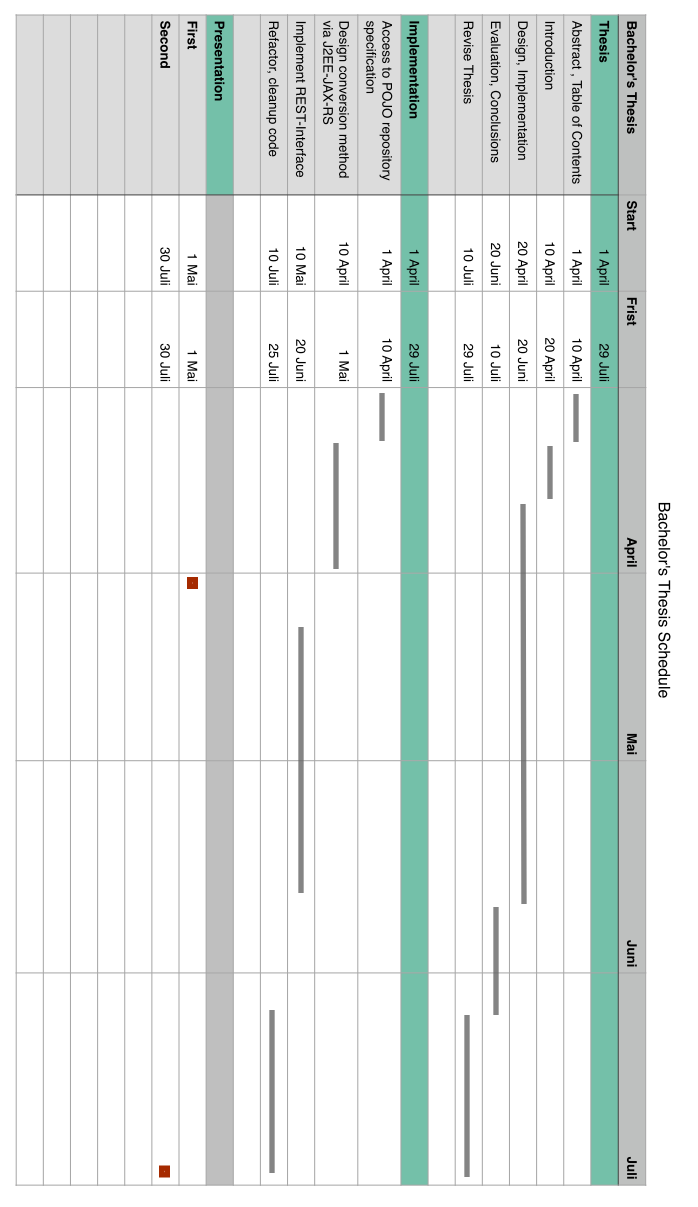
\includegraphics[width=0.93\textwidth]{resources/images/schedule.png}
	\label{fig:schedule}
\end{figure}



%\sidenote{Outlook}


%    \begin{quote}
%    "`\begin{CJK}{UTF8}{gbsn}不闻不若闻之,闻之不若见之,见之不若知之,知之不若行之;学至于行之而止矣。\end{CJK}"' -
%    \textit{Xunzi, Chinese philosopher (about 300-230 BC)}
%
%    "`not hearing is not as good as hearing, hearing is not as good as
%       seeing, seeing is not as good as mentally knowing, mentally knowing is
%       not as good as acting; true learning continues up to the point that
%       action comes forth [or, only when a thing produces action can it be said
%      to have been truly learned]"'
%    \end{quote}

%\cleardoublepage
%\chapter*{Zusammenfassung}\label{sec:zusammenfassung}
%\sidenote{Einleitung und Problemstellung}
%\lipsum[6]

%\sidenote{Verwandte Arbeiten und Forschungsfragen}
%\lipsum[6]

%\sidenote{Wissenschaftlicher Beitrag}
%\lipsum[6]

%\sidenote{Zusammenfassung}
%\lipsum[6]
\cleardoublepage
